% Adapted from the 5writing English MCM LaTeX template for this contest.
\documentclass[11pt,a4paper]{article}
\usepackage[margin=19mm,headheight=14pt]{geometry}
\ifdefined\XeTeXversion
  \usepackage{fontspec}
  \setmainfont{TeX Gyre Termes}
  \setsansfont{TeX Gyre Heros}
\else
  \usepackage[T1]{fontenc}
  \usepackage{mathptmx}
\fi
\usepackage{amsmath,amssymb,booktabs,graphicx,tabularx,xcolor}
\usepackage[colorlinks=true,linkcolor=teal,citecolor=teal,urlcolor=teal]{hyperref}
\urlstyle{same}
\definecolor{teal}{HTML}{007C83}
\setlength{\parindent}{0pt}
\setlength{\parskip}{5pt}
\setlength{\tabcolsep}{5pt}
\renewcommand{\arraystretch}{1.13}
\renewcommand{\baselinestretch}{1.025}
\makeatletter
\renewcommand\normalsize{\@setfontsize\normalsize{11.1pt}{13.4pt}}
\let\tableinput\@@input
\makeatother
\normalsize
\setlength{\emergencystretch}{1em}
\setlength{\abovedisplayskip}{7pt}
\setlength{\belowdisplayskip}{7pt}
\newcommand{\ES}{\operatorname{ES}}
\newcommand{\Pten}{\operatorname{P10}}
\newcommand{\Pninety}{\operatorname{P90}}
\newcommand{\PaperTitle}{SafeInvest: Horizon-Aware Allocation with Cost-Gated Portfolio Updates}
\newcommand{\PaperDate}{19 October 2026}
\newcommand{\PaperAuthors}{Huang Sinan, Cai Xunzhi, Lin Zihan}
\newcommand{\PaperTeam}{Fen8FenQian}
\newcommand{\AITools}{OpenAI ChatGPT/Codex}
\newcommand{\BalancedGrowth}{4.15}
\newcommand{\BalancedPten}{1.64}
\newcommand{\BalancedMedianLoss}{30.58}
\newcommand{\BalancedPninety}{48.02}
\newcommand{\BalancedVolatility}{10.76}
\newcommand{\BalancedTrades}{35.34}
\newcommand{\BalancedTailLoss}{59.31}
\newcommand{\BalancedCost}{0.5834}
\newcommand{\EqualGrowth}{3.38}
\newcommand{\EqualPten}{1.50}
\newcommand{\EqualMedianLoss}{22.30}
\newcommand{\EqualPninety}{39.53}
\newcommand{\EqualVolatility}{8.24}
\newcommand{\EqualTrades}{100.00}
\newcommand{\EqualTailLoss}{50.83}
\newcommand{\EqualCost}{0.6603}
\newcommand{\AnnualGrowth}{4.02}
\newcommand{\AnnualPten}{1.67}
\newcommand{\AnnualMedianLoss}{30.30}
\newcommand{\AnnualPninety}{48.12}
\newcommand{\AnnualVolatility}{10.59}
\newcommand{\AnnualTrades}{100.00}
\newcommand{\AnnualTailLoss}{60.21}
\newcommand{\AnnualCost}{0.7973}
\newcommand{\HoldGrowth}{4.27}
\newcommand{\HoldPten}{1.42}
\newcommand{\HoldMedianLoss}{36.05}
\newcommand{\HoldPninety}{59.15}
\newcommand{\HoldVolatility}{13.34}
\newcommand{\HoldTrades}{0.00}
\newcommand{\HoldTailLoss}{65.98}
\newcommand{\HoldCost}{0.1631}
\newcommand{\CostSaving}{26.83}
\newcommand{\GrowthGain}{0.78}
\newcommand{\RiskIncrease}{8.49}
\newcommand{\AnnualGrowthGain}{0.13}
\newcommand{\HoldRiskReduction}{11.13}
\newcommand{\HoldGrowthLoss}{0.11}
\newcommand{\IncludingInitialTrades}{37.50}
\newcommand{\DoubleGrowth}{4.13}
\newcommand{\DoubleTrades}{28.68}
\newcommand{\DoubleCost}{1.0668}
\newcommand{\SeverePeak}{162.33}
\newcommand{\SevereTerminal}{56.50}
\newcommand{\SevereLoss}{65.19}
\newcommand{\SevereGrowth}{-1.88}
\newcommand{\ReviewThreshold}{63.85}
\newcommand{\GrowthCILower}{0.325}
\newcommand{\GrowthCIUpper}{1.184}
\newcommand{\GrowthCIFamilyLower}{0.098}
\newcommand{\GrowthCIFamilyUpper}{1.372}
\newcommand{\LossCILower}{5.203}
\newcommand{\LossCIUpper}{13.365}
\newcommand{\LossCIFamilyLower}{3.399}
\newcommand{\LossCIFamilyUpper}{15.735}

\hypersetup{pdftitle={SafeInvest: Horizon-Aware Allocation with Cost-Gated Portfolio Updates},pdfauthor={\PaperAuthors}}
\begin{document}
\begin{center}
{\large 2026 MCM Senior Group \textbar\ Problem A}\par
\vspace{6pt}
{\LARGE\bfseries\color{teal}\PaperTitle\par}
\vspace{8pt}
{\PaperAuthors}\par
\PaperTeam\quad\textbar\quad\PaperDate
\end{center}
\vspace{4pt}
\begin{center}\textbf{Abstract}\end{center}
SafeInvest must choose suitable investments, avoid unnecessary trading, and recognize when automated advice should stop. We develop three horizon-specific portfolios using a convex expected-log-growth problem constrained by tail log drawdown. A separate execution rule moves partially toward the strategic allocation only when the estimated benefit exceeds transaction costs and a safety margin. Suitability is assessed at each customer's actual horizon using out-of-fold loss outcomes, conservative probability bounds, and a doubled-cost stress test. The selected, frozen Plan A assigns customers B and C to Conservative, E to Balanced, and A and D to human review.

All development uses 120 complete scenarios. A single frozen evaluation uses the remaining 60; its saved outputs provide the evidence reported here. At 30 years and a 0.25\% transaction cost, Balanced A delivers a median real annual growth of \BalancedGrowth\%, compared with \EqualGrowth\% for annual equal-weight rebalancing. Its 90th-percentile maximum drawdown is also higher: \BalancedPninety\% versus \EqualPninety\%. Against annual rebalancing to the same strategic allocation, the execution rule reduces mean real fees by \CostSaving\% and trades at \BalancedTrades\% of subsequent annual reviews. A severe scenario nevertheless loses \SevereLoss\% from peak to trough. The evidence supports selective, explainable automation with explicit escalation; it does not establish a guarantee against loss or universal superiority over the baseline.

\section{Decision Problem and Evidence}
The advisor invests in equities, government bonds, and Treasury bills. Its responsibilities are linked: define Conservative, Balanced, and Growth products; match customers to a product or a human advisor; and choose among keeping holdings, rebalancing, changing the current target, and requesting human review. Optimizing returns alone does not address these service decisions.

The supplied data comprise 180 independent synthetic scenarios, each with 30 annual observations of asset returns and inflation. They are based on selected US series from the JST Macrohistory Database, Release 6, as described in the problem statement \cite{problem,jst}. Scenario numbers identify simulated paths, not historical episodes. We retain each complete path as one statistical unit and use the first $H$ periods when evaluating a customer with horizon $H$.

Scenarios 1--120 form the development partition; scenarios 121--180 are reserved for the final evaluation. The latter was executed once on 17 October 2026 after model settings, customer assignments, and comparators were frozen. The final decision retains calibrated Plan A because subsequent development candidates did not satisfy the complete replacement criteria. Neural-network experiments are therefore outside the submitted strategy. Report preparation uses saved summaries and verification records only.

Our design separates three questions: what long-run allocation is appropriate, whether the customer can be served automatically, and whether an immediate trade is worth its cost. This makes the recommendation auditable and permits a justified refusal to automate.

\clearpage
\section{Accounting, Assumptions, and Performance Measures}
\subsection{A causal, self-contained investment account}
Wealth starts at 100 units, entirely in bills. Portfolios are long-only and fully invested: $w_i\geq0$ and $\sum_i w_i=1$. There are no contributions, withdrawals, leverage or taxes, no fees other than the stated transaction cost, and no assumed terminal liquidation. A decision for period $t$ uses only observations through period $t-1$ of that scenario, so every reported path is causal. Bills supply liquidity, but their real return can be negative: preservation of purchasing power is not assumed.

Let $h^-_{i,t}$ be pre-trade nominal holdings, $V^-_t=\sum_i h^-_{i,t}$, and $p_{i,t}=h^-_{i,t}/V^-_t$. A target $w_t$ moves the following amount and incurs the following fee at rate $c$:
\begin{equation}
Q_t=\frac{V^-_t}{2}\lVert w_t-p_t\rVert_1,\qquad F_t=cQ_t,\qquad
h^+_{i,t}=(V^-_t-F_t)w_{i,t}.
\label{eq:fees}
\end{equation}
The one-half factor counts each transferred amount once instead of charging the sale and the purchase separately: at $c=0.25\%$, moving 20 units from bills to equities costs 0.05 units. Turnover is measured against pre-fee wealth, the fee is deducted before that period's returns, and the remainder is placed at the target. We state this convention rather than solve for an implicit trade that reproduces the target after the fee. The initial allocation is charged the same way, starting from an all-bill account.

For nominal return $r_{i,t}$ and inflation $\pi_t$, define real return $\rho_{i,t}$, cumulative price index $I_t$, and year-end real wealth $W_t$ by
\begin{equation}
\rho_{i,t}=\frac{1+r_{i,t}}{1+\pi_t}-1,\qquad
I_t=\prod_{k=1}^t(1+\pi_k),\qquad
W_t=\frac{\sum_i h^+_{i,t}(1+r_{i,t})}{I_t}.
\end{equation}
Pending human review means existing assets stay invested and automatic trades stop; no unobserved intervention, liquidation or recovery is credited to the algorithm.

\subsection{Growth, ordinary fluctuation, and unusually large loss}
For a scenario with horizon $H$, real compound annual growth is
\begin{equation}
G=\left(\frac{W_H}{100}\right)^{1/H}-1.
\end{equation}
Maximum drawdown measures loss from a previous real-wealth peak. Let $Z_j$ contain the initial wealth, each post-fee/pre-return wealth mark, and each year-end wealth mark. Then
\begin{equation}
D=\max_j\left(1-\frac{Z_j}{\max_{k\leq j}Z_k}\right).
\label{eq:drawdown}
\end{equation}
Including the post-fee marks keeps trading losses visible instead of hiding them between annual observations. The measure is oriented so that larger values mean a greater loss. A stated customer tolerance $L$ is evaluated through the event $D>L$; it is a preference threshold, not a guaranteed loss limit.

The brief asks for ordinary fluctuation and unusually large loss to be separated, both in purchasing-power terms; every measure below is real. Ordinary fluctuation is the annual volatility $\sigma$, the sample standard deviation of net real annual returns. Unusually large loss is reported as the 90th percentile of $D$ and as the 90\% drawdown CVaR, which averages the worst 10\% of scenario drawdowns, with fractional boundary weights where needed. CVaR is not a percentile, and the two tail figures are therefore not interchangeable. Across scenarios we report median $G$, $\Pten(G)$, median $D$ and $\Pninety(D)$, and the cross-scenario median of $\sigma$ summarizes variability within a path, not dispersion across paths. Terminal-loss probability is the share of scenarios with $W_H<100$.

The main trading frequency is the fraction of reviews in periods $2,\ldots,H$ that execute a trade, excluding the compulsory initial allocation; the rate including it is reported where relevant. Mean real fees accumulate inflation-adjusted fees over the horizon in units of initial wealth 100. Review incidence is the fraction of scenarios that ever request human review.

\clearpage
\section{Strategic Portfolios and Customer Suitability}
\subsection{A convex allocation problem for each horizon}
For $N$ training paths and a target $w$ restored every year, the largest cumulative log loss over any contiguous interval is
\begin{equation}
Y_s(w)=\max_{0\leq u\leq v\leq H}\left\{-\sum_{t=u+1}^{v}\log(1+\rho_{s,t}^{\mathsf T}w)\right\}.
\end{equation}
The empty interval contributes zero. On this cost-free, annually restored model an ordinary maximum drawdown equals $1-\exp(-Y_s)$, but the expectation does not commute with that transform: $\ES(Y)$ does not generally give $\ES(D)$. We therefore constrain the quantity we can compute and report the resulting drawdown afterwards.

Using the variational representation of expected shortfall \cite{cvar},
\begin{equation}
\ES_\alpha(Y)=\min_z\left[z+\frac{1}{N(1-\alpha)}\sum_{s=1}^{N}(Y_s-z)_+\right],\quad \alpha=0.90,
\end{equation}
we choose the strategic anchor $w^*$ by solving
\begin{align}
\min_w\quad &-\frac{1}{NH}\sum_{s=1}^{N}\sum_{t=1}^{H}\log(1+\rho_{s,t}^{\mathsf T}w)\\
\text{subject to}\quad &\ES_{0.90}(Y(w))\leq qR_{\rm ref},\quad w\geq0,\quad\mathbf{1}^{\mathsf T}w=1.
\label{eq:strategy}
\end{align}

For each horizon, $R_{\rm ref}$ is the training log-drawdown expected shortfall of a stated reference allocation: $(.20,.30,.50)$ for Conservative, $(.50,.35,.15)$ for Balanced and $(.75,.20,.05)$ for Growth. The multiplier $q\in\{.75,.85,.95\}$ scales the training budget and is chosen in Section~3.2, while the validation target stays at $R_{\rm ref}$. Conservative additionally requires $w_{\rm bill}\geq0.40$. The three products thus differ both in risk budget and, for Conservative, in a liquidity floor.

Negative log growth and the maximum of interval log losses are convex on the valid-return domain, so \eqref{eq:strategy} is a convex subproblem. We solve it with a Kelley cutting-plane linear program: supporting hyperplanes generate objective lower bounds, feasible weights upper bounds, and the loop stops at a gap of $10^{-6}$, with risk tolerance $10^{-8}$ and at most 300 iterations, starting from a 231-point 5\% simplex grid that also supplies a comparison objective. Primal solutions and dual multipliers are saved so that feasibility and duality balance can be re-checked. An infeasible risk budget is recorded and never repaired by quietly relaxing it. These certificates cover the strategic subproblem only; they say nothing about the optimality of the trading and escalation layer.

\subsection{Development selection before freezing}
Selection happens before the holdout is touched. Nested validation uses five outer folds of complete paths, 96 scenarios to train and 24 to validate, and three inner folds of 64 and 32 inside each outer training set, so every choice is scored on data the candidate was not fitted to. Candidates pair $q\in\{.75,.85,.95\}$ with execution curvature $\gamma\in\{4,12\}$. Comparing them on held-out outcomes rather than on training fit limits the selection bias that repeated comparisons introduce \cite{cawley}.

A candidate is feasible on validation only if four conditions hold. Pooled log-drawdown expected shortfall at 90\% must not exceed $R_{\rm ref}$ plus 0.005 in log units; that slack is fixed in advance and does not follow $q$. The median and the 10th percentile of annual real growth must not fall more than 0.001 and 0.002 below fee-paying annual rebalancing to the same anchor. Reviews, and hence the trades they permit, must be requested in at most 10\% of validation scenarios. Among feasible candidates we maximize the mean of $\log(1+G)$. If none is feasible, the least-violating candidate is retained as a diagnostic and marked unusable rather than presented as a selection. All three products selected $q=0.95$ and $\gamma=4$ on the full development set, after which the anchors and the customer assignments were frozen.

\subsection{Frozen allocations and an explicit refusal option}
Table~\ref{tab:weights} gives the frozen anchors at the five horizons that appear in the questionnaire. A product name does not imply one allocation for every customer: Conservative is nearly invariant to the horizon, holding 70--74\% in bills throughout, while Balanced and Growth move bills into bonds as the horizon lengthens, and the 30-year Growth solution reaches the boundary with no bills at all. The response is not monotone in the middle of the range, because each anchor is fitted separately at its own horizon. These are model outputs under the stated data and constraints, not general investment prescriptions.

\begin{table}[h!]
\centering
\caption{Frozen strategic equity / bond / bill weights (\%) from the full-development refit; rounding may make totals differ from 100.}
\label{tab:weights}
\begin{tabular}{rlll}\toprule
$H$ & Conservative & Balanced & Growth\\\midrule
\tableinput{generated/weights.tex}
\bottomrule\end{tabular}
\end{table}

For horizon $H$ and tolerance $L$ we count out-of-fold paths whose complete execution policy breaches $D>L$; with $k$ breaches among $n=120$, the one-sided Clopper--Pearson upper bound is
\begin{equation}
U=\operatorname{Beta}^{-1}(1-\delta;k+1,n-k),\qquad
\delta=0.05/440,
\end{equation}
with $U=1$ when $k=n$. The family of 440 is fixed before screening and covers five profiles, 11 distinct product-or-programme choices, four liquidity conventions and two cost levels. Automatic service requires $U\leq0.20$ at the base cost and at doubled cost alike. Because the out-of-fold policies are refitted on overlapping training sets, $U$ is a conservative screening diagnostic rather than a coverage guarantee for the final refitted policy, and the 20\% ceiling is a service assumption, not a stated customer preference.

Two further rules follow from the questionnaire. A high-liquidity profile requires a strategic bill weight of at least 40\% in every relevant development fold; the condition is checked for any eligible product, so such a profile is not forced into the product named Conservative, and the target is not a cash floor maintained after market drift. Growth is offered only from a 15-year horizon upwards, and P90 drawdown must be ordered Conservative $\leq$ Balanced $\leq$ Growth. Among the pairs that clear every rule, the one with the highest out-of-fold median growth is recommended; if none clears them, the profile goes to human review.

Table~\ref{tab:suitability} applies these rules pair by pair. For A and D no product comes close, so referral is the model's answer rather than a default. B and C clear only through Conservative, and C's Balanced alternative fails the ceiling on 17 breaches. E has two qualifying pairs; Balanced wins on out-of-fold median growth, 4.22\% against 2.71\%. All three served profiles also clear the doubled-cost test.

\begin{table}[h!]
\centering
\caption{Screening of every profile--product pair on development data: breaching paths $k/120$ and the bound $U$ (\%). Bold marks a pair that also clears the liquidity, horizon, ordering and doubled-cost rules.}
\label{tab:suitability}
\begin{tabular}{lcclccccccc}\toprule
Profile & $H$ & Tol.\,(\%) & Liquidity & \multicolumn{2}{c}{Conservative} & \multicolumn{2}{c}{Balanced} & \multicolumn{2}{c}{Growth} & Assigned\\
\cmidrule(lr){5-6}\cmidrule(lr){7-8}\cmidrule(lr){9-10}
 & & & & $k/120$ & $U$ & $k/120$ & $U$ & $k/120$ & $U$ & \\\midrule
\tableinput{generated/suitability.tex}
\bottomrule\end{tabular}
\end{table}

\clearpage
\section{Annual Execution and Human Escalation}
\subsection{Candidate trades and the cost gate}
At each annual review, the advisor checks for escalation before considering a trade. Let $p$ denote current portfolio weights and $w^*$ the frozen strategic anchor for the investment horizon. The five candidates are
\begin{equation}
w_\lambda=p+\lambda(w^*-p),\qquad
\lambda\in\{0,.25,.50,.75,1\}.
\end{equation}
Here, $\lambda=0$ keeps holdings and $\lambda=1$ restores the anchor. Training returns supply the mean $\mu$ and regularized covariance $\Sigma=0.75S+0.25\operatorname{diag}(S)+10^{-10}I$. The tracking score and fractional trading cost are
\begin{equation}
A(w)=1+\mu^{\mathsf T}w^*-\frac{\gamma}{2}(w-w^*)^{\mathsf T}\Sigma(w-w^*),
\qquad f_\lambda=\frac{c}{2}\lVert w_\lambda-p\rVert_1.
\end{equation}
The return term is shared across candidates; the quadratic term penalizes departure from the anchor. If any score is nonpositive or nonfinite, the advisor requests human review. Otherwise, it selects $j$ maximizing $(1-f_\lambda)A(w_\lambda)$ and accepts a trade only if
\begin{equation}
\frac{A(w_j)-A(p)}{A(w_j)}>f_j+0.0001.
\label{eq:gate}
\end{equation}
The extra 0.0001 is a one-basis-point safety margin. If the selected candidate fails this strict gate, holdings are kept; lower-ranked candidates are not tried. This score measures tracking benefit, not a guaranteed increase in future wealth.

\subsection{Four observable actions}
Before trading, the advisor compares observed real drawdown with the training-based threshold
\begin{equation}
\tau=\operatorname{clip}\!\left(1.5\,\Pninety(D_{\rm train,annual}),\ 0.10,\ 0.75\right),
\end{equation}
where $D_{\rm train,annual}$ comes from fee-paying annual rebalancing to the same anchor. For 30-year Balanced A, $\tau=\ReviewThreshold\%$. Table~\ref{tab:actions} distinguishes the four actions. Escalation takes priority over candidate selection; while review is pending, the engine holds existing assets and suspends automatic trading.

\begin{table}[h!]
\centering
\caption{Annual action rules. Accepted trades are classified against the previously recorded execution target, not necessarily the strategic anchor.}
\label{tab:actions}
\begin{tabularx}{\linewidth}{lX}\toprule
Action & Decision rule\\\midrule
1. Keep holdings & The selected step is zero or fails Equation~\eqref{eq:gate}; no trade fee is charged.\\
2. Rebalance & The accepted trade restores the recorded execution target.\\
3. Change target & The accepted trade sets a different execution target; $w^*$ remains fixed.\\
4. Request human review & Observed drawdown reaches $\tau$, or a candidate score is invalid; existing assets remain invested.\\
\bottomrule\end{tabularx}
\end{table}

\subsection{Customer-facing explanation}
Every accepted adjustment uses this 20-word explanation, within the required 50-word limit:
\begin{quote}
``This adjustment moves your investments toward the strategic allocation. Its estimated risk-adjusted benefit exceeds trading costs. Investment losses remain possible.''
\end{quote}

\clearpage
\section{Final Evaluation Results}
\subsection{Higher growth comes with greater drawdown}
Table~\ref{tab:performance} compares policies on the same 60 final scenarios, charging 0.25\% of money moved. Equal-weight annual rebalancing is the required baseline; same-anchor annual and hold controls isolate execution effects.

\begin{table}[h!]
\centering
\caption{Thirty-year final outcomes across 60 scenarios (\%). $G$: net real CAGR; $D$: maximum real drawdown. Trade rate excludes initial allocation.}
\label{tab:performance}
\begin{tabular}{lrrrrr}\toprule
Policy & Med. $G$ & P10 $G$ & Med. $D$ & P90 $D$ & Trades\\\midrule
\tableinput{generated/performance.tex}
\bottomrule\end{tabular}
\end{table}

\begin{figure}[h!]
\centering
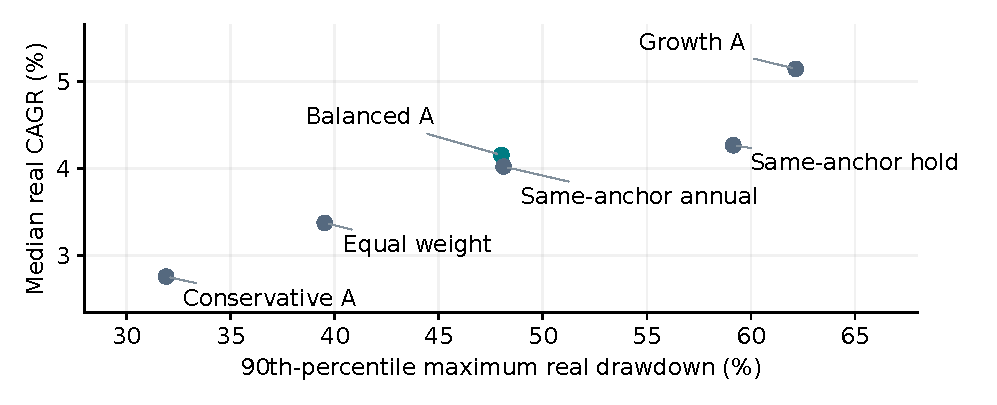
\includegraphics[width=\linewidth]{figures/risk_growth.pdf}
\caption{Thirty-year median growth versus P90 drawdown across 60 scenarios at the base fee. P90 is not a loss guarantee.}
\label{fig:riskgrowth}
\end{figure}

Balanced A gained \GrowthGain{} percentage points (pp) of median growth over equal weight, with \RiskIncrease{} pp more P90 drawdown (Figure~\ref{fig:riskgrowth}). Its median annual volatility was \BalancedVolatility\%, compared with \EqualVolatility\% for equal weight.

\begin{table}[h!]
\centering
\caption{Paired bootstrap comparisons, Balanced A minus equal weight (pp); 4,000 complete-scenario resamples.}
\label{tab:paired}
\begin{tabular}{lrrr}\toprule
Metric & Difference & 95\% interval & Family-adjusted 95\%\\\midrule
Median $G$ & +\GrowthGain & [\GrowthCILower, \GrowthCIUpper] & [\GrowthCIFamilyLower, \GrowthCIFamilyUpper]\\
P90 $D$ & +\RiskIncrease & [\LossCILower, \LossCIUpper] & [\LossCIFamilyLower, \LossCIFamilyUpper]\\
\bottomrule\end{tabular}
\end{table}

Family adjustment covers 20 nonbaseline policies within each endpoint, horizon, and cost; it does not cover the whole adaptive research process.

Against same-anchor annual rebalancing, Balanced A gained \AnnualGrowthGain{} pp of median growth with nearly unchanged P90 drawdown. Mean real fees fell \CostSaving\%, from \AnnualCost{} to \BalancedCost{}. Its trade rate was \BalancedTrades\% (\IncludingInitialTrades\% including initial allocation). Relative to holding the anchor, P90 drawdown fell \HoldRiskReduction{} pp and median growth fell \HoldGrowthLoss{} pp. These comparisons favour selective rebalancing when fees and tail losses both matter.

\subsection{Customer outcomes at their actual horizons}
Table~\ref{tab:customers} uses each customer's actual horizon and frozen assignment. A and D were referred for human review; dashes indicate no automated investment path. Breaches mean maximum drawdown exceeded the customer's stated tolerance.

\begin{table}[h!]
\centering
\caption{Final customer outcomes (growth and drawdown in \%; 60 scenarios).}
\label{tab:customers}
\begin{tabular}{crrrrrl}\toprule
Customer & $H$ & Med. $G$ & P10 $G$ & Med. $D$ & P90 $D$ & Breaches\\\midrule
\tableinput{generated/customers.tex}
\bottomrule\end{tabular}
\end{table}

\begin{table}[h!]
\centering
\caption{Customer risk and trading. Terminal loss means final real wealth below 100; trade rates exclude initial allocation.}
\label{tab:customerrisk}
\begin{tabular}{crlr}\toprule
Customer & Median volatility (\%) & Terminal losses & Trade rate (\%)\\\midrule
\tableinput{generated/customer_risk.tex}
\bottomrule\end{tabular}
\end{table}

For B, P90 drawdown exceeded the 25\% tolerance, with breaches in 7 of 60 scenarios. Eligibility screens breach probability, rather than imposing a guaranteed loss limit. E's negative P10 growth and 9 terminal losses highlight the risk of its six-year horizon despite positive median growth. B, C, and E requested human review in 2, 3, and 0 scenarios, respectively. All assignments remained unchanged after final evaluation.

\subsection{A severe path exposes the limits of escalation}
In scenario 155, Balanced A peaked at \SeverePeak{} in year 6 and ended at \SevereTerminal{} (Figure~\ref{fig:severe}). Its \SevereLoss\% maximum drawdown and \SevereGrowth\% real CAGR show the limits of annual escalation.

\begin{figure}[h!]
\centering
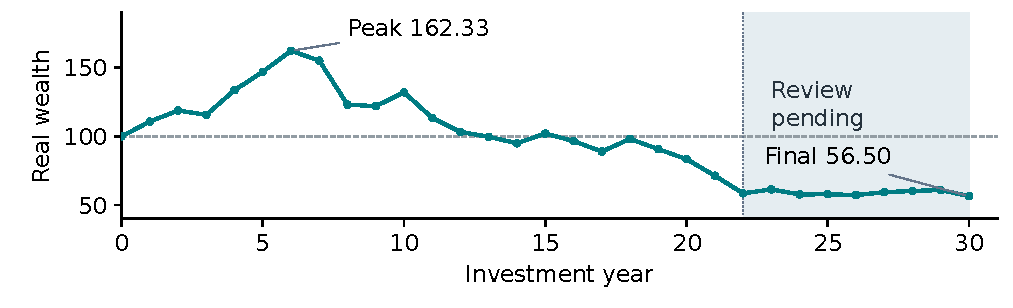
\includegraphics[width=\linewidth]{figures/severe_path.pdf}
\caption{Saved real wealth for scenario 155, starting from 100. Lines join year-end observations; shading marks pending review, beginning before year 23.}
\label{fig:severe}
\end{figure}

Six post-initial trades preceded the review request before the year-23 return. Automatic trading then stopped, but the existing holdings remained exposed. Across all 60 Balanced paths, drawdown CVaR90 was \BalancedTailLoss\%, versus P90 drawdown of \BalancedPninety\%.

\clearpage
\section{Sensitivity and Reliability}
\subsection{Transaction-cost stress with the policy frozen}
The saved final cost sweep changes the fee rate while keeping the strategic model and customer assignments fixed. The cost gate still responds to the fee it faces. Table~\ref{tab:cost} and Figure~\ref{fig:cost} therefore describe a fixed decision rule under different execution costs, not a refitted strategy.

\begin{table}[h!]
\centering
\caption{Thirty-year Balanced A under alternative transaction costs. Growth and drawdown are in \%; fees are real wealth units.}
\label{tab:cost}
\begin{tabular}{rrrrrr}\toprule
Cost (\%) & Med. $G$ & P10 $G$ & P90 $D$ & Mean fees & Trades (\%)\\\midrule
\tableinput{generated/costs.tex}
\bottomrule\end{tabular}
\end{table}

\begin{figure}[h!]
\centering
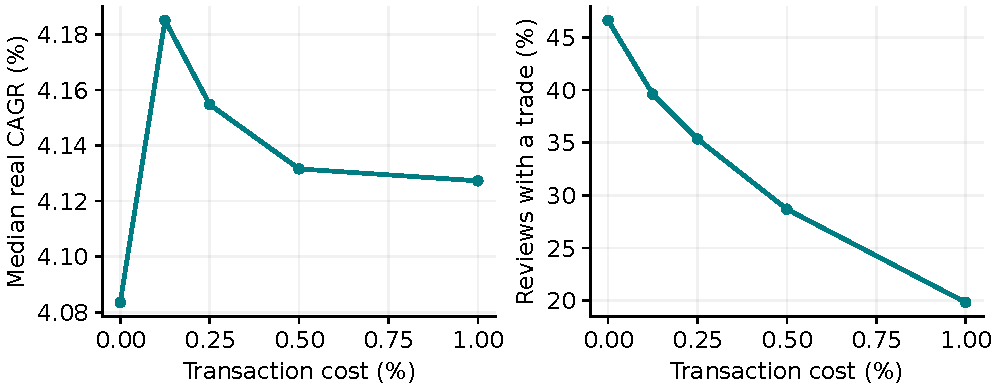
\includegraphics[width=\linewidth]{figures/cost_sensitivity.pdf}
\caption{Higher fees suppress trading; growth need not fall monotonically because the actions also change.}
\label{fig:cost}
\end{figure}

Doubling the fee to 0.50\% reduces the trading rate to \DoubleTrades\%, while median real growth remains \DoubleGrowth\%. Mean real fees rise to \DoubleCost{}. Small nonmonotonic growth differences should not be interpreted as a benefit from charging fees: changed trades lead to changed exposures on the same finite set of scenarios.

\subsection{What is verified, and what remains uncertain}
Saved checks covered 286,920 transitions, 780 equal-weight scalar-reference cases, and five customer assignments. Maximum absolute reconstructed year-end holding error was $3.64\times10^{-12}$ nominal wealth units. These checks support accounting consistency, not predictive reliability.

Synthetic data and only 60 independent final paths limit generalization and tail-risk precision; testing five fees does not add independent paths. Annual reviews miss within-year drawdowns, and the cost-free strategic risk proxy differs from realized execution risk. Bill weights can drift below targets. Withdrawals, taxes, additional frictions, and effective human intervention are unmodeled.

\clearpage
\section{Recommendation and Conclusions}
We retain the frozen calibrated Plan A as the final submission strategy. Its three products use horizon-specific strategic allocations, and its execution layer trades only when a local benefit estimate clears costs and a safety margin. Customer screening is separate from return maximization: B and C receive Conservative, E receives Balanced, and A and D are referred to a human advisor.

The main empirical result is a trade-off. Balanced A improves 30-year median real growth over annual equal weight, but also produces greater tail drawdown. A fairer test of the execution layer compares the same anchor: selective trading cuts mean real fees by \CostSaving\% relative to annual restoration, with similar tail drawdown in the final sample. Conversely, the severe path demonstrates that even an observed review trigger does not stop an ongoing loss.

SafeInvest should explain its targets, disclose losses in real purchasing-power terms, state that assets remain invested during review, and retain a refusal option. Neither the service ceiling nor the training risk constraint guarantees protection. Faster human response and stronger downside controls remain future research questions requiring independent evaluation.

\subsection*{Reproducibility and attribution}
The implementation preserves the frozen model, development selection record, one-time final-evaluation lock, and saved comparator outputs. Tables and figures are generated directly from those records. Supplementary source code is a separate submission artifact; this report is self-contained.

The problem statement and supplied scenario data are credited to the 2026 MCM Senior Group organizers and their stated underlying JST source \cite{problem,jst}. We acknowledge the supplied materials' Creative Commons Attribution--NonCommercial--ShareAlike 4.0 license. Derived data displays in this report retain that attribution and are shared under the same terms. All returns in this report describe the supplied synthetic experiment, not forecasts of future asset performance.

\begin{thebibliography}{9}
\bibitem{problem} 2026 MCM Senior Group Organizers. \emph{Problem A: SafeInvest: Building a Trustworthy Robo-Advisor}. Competition problem statement and supplied scenario data, 2026.
\bibitem{cvar} R. T. Rockafellar and S. Uryasev. \emph{Optimization of Conditional Value-at-Risk}. Author manuscript, 5 September 1999. \url{https://sites.math.washington.edu/~rtr/papers/rtr179-CVaR1.pdf}.
\bibitem{cawley} G. C. Cawley and N. L. C. Talbot. On over-fitting in model selection and subsequent selection bias in performance evaluation. \emph{Journal of Machine Learning Research}, 11:2079--2107, 2010. \url{https://www.jmlr.org/papers/v11/cawley10a.html}.
\bibitem{jst} O. Jord\`a, M. Schularick, and A. M. Taylor. \emph{JST Macrohistory Database}. Source series identified in the competition statement as Release 6. \url{https://www.macrohistory.net/database/}. Accessed 19 October 2026.
\end{thebibliography}

\section*{Use of AI Tools}
\AITools{} assisted with code development, analysis, drafting, and document checks. Numerical claims in this report are drawn from saved experiment outputs and frozen model settings; the report-building step did not refit a model or rerun the final evaluation. AI-generated explanations and prose require review by the named team members before submission. The authors remain responsible for the correctness, originality, attribution, and final submitted content.
\end{document}
